\section{Teoretická časť}

\subsection{Odporúčacie systémy}
\label{sec:odporucacie systemy}
 Odporúčacie systémy predstavujú súbor softvérových nástrojov a techník, ktoré poskytujú používateľovi odporúčania ohľadom daného súboru položiek. Odporúčania súvisia s rôznymi rozhodovacími procesmi, ako napríklad akú položku kúpiť, akú hudbu počúvať alebo aké online noviny  čítať. \cite{rs1} Dalo by sa teda povedať, že ich hlavným cieľom je odporučiť danému používateľovi jemu relevantné položky. "Položka" je termín, ktorý označuje čo konkrétne daný odporúčací systém odporúča používateľom. Vzhľadom nato, že odporúčania sú väčšinou personalizované, rôzny používatelia dostávajú rozličné odporúčania. Existujú aj nepersonalizované odporúčania. Tie fungujú na jednoduchšom princípe a je ľahšie ich generovať. Typickým príkladom sú rebríčky, ktoré obsahujú výber top 10 najobľúbenejších položiek. Personalizované odporúčania v ich najjednoduchšej forme sú zoradené zoznamy položiek.
 
Keď sa pozrieme na dôležitosť týchto systémov, v určitých odvetviach zohrávajú dôležitú rolu. Väčšina veľkých internetových služieb ako Amazon, YouTube, Netflix, Google, Tripadvisor či IMDb, majú vyvinuté svoje vlastné odporúčacie systémy, ktoré dlhodobo pomáhajú zlepšovať ich výsledky, ale aj UX. Tak isto aj mnoho mediálnych firiem už dnes vyvíja odporúčacie systémy, ktoré potom nasadzujú a používajú ako časť služby, ktorú poskytujú svojim odoberateľom. Netflix v roku 2009 ocenil tím programátorov, ktorý ako prvý úspešne zefektívnil ich odporúčací systém o takmer 10\%, cenou 1 milión dolárov. To len podčiarkuje ich významnosť a fakt, že svetové firmy do tejto technológie investujú nemalé finančné prostriedky.  \\

\subsubsection{Základné funkcie}
Existuje viacero dôvodov, prečo môžu poskytovatelia služieb chcieť túto technológiu využiť: 
 \begin{itemize}[leftmargin=*]
{\bf \item Zvýšenie predaja} - najdôležitejšia funkcia pre komerčný odporúčací systém, je samozrejme zvýšenie počtu predaných položiek. Čím efektívnejší je, tým lepšie výsledky firme generuje.

{\bf \item Predávať rôznorodý tovar} - ďalšia významná funkcia je umožniť používateľovi vybrať si položky, ktoré by bez odporúčania ťažšie našiel.
 
{\bf \item Zvýšiť spokojnosť používateľa} - dobre fungujúci odporúčací systém, vie zlepšiť aj celkový \acrshort{ux}, čo v konečnom dôsledku zabezpečí, že používateľ bude odporúčania rád využívať.

{\bf \item Zvýšiť vernosť používateľa} - akonáhle používateľ zaregistruje, na základe presných odporúčaní, že ho služba "pozná", nadobudne pocit, že ho považuje za hodnotného zákazníka a bude sa rád vracať.
	
{\bf \item Lepšie rozumieť tomu, čo zákazník chce} - pomocou zbierania rôznych používateľských preferencií a následného analyzovania, vedia firmy lepšie reagovať na trh a zmeny na ňom a tým prispôsobovať svoj sortiment potrebám trhu.  \newline

\end{itemize} 


\subsubsection{Základné pojmy}
Všeobecná klasifikácia dát použitých v odporúčacích systémoch rozlišuje 3 druhy objektov.
 \begin{itemize}[leftmargin=*]
{\bf \item Položky} - sú objekty ktoré sú odporúčané. Môžu byť charakterizované ich zložitosťou a ich hodnotou alebo užitočnosťou. Hodnota môže byť kladná, ak je položka pre používateľa užitočná, alebo záporná, ak položka nie je vhodná a používateľ pri jej výbere urobil nesprávne rozhodnutie.
{\bf \item Používatelia} - môžu mať veľmi rozdielne ciele a vlastnosti. S cieľom personalizovať odporúčania a interakciu s počítačom, odporúčacie systémy využívajú množstvo informácií o používateľoch. Tieto informácie môžu byť štrukturované viacerými spôsobmi a výber, ktoré informácie treba modelovať systémom, záleží od zvolenej techniky. 
{\bf \item Transakcie} - všeobecne ich označujeme ako zaznamenanú interakciu medzi používateľom a odporúčacím systémom. Sú to dáta podobného typu ako logy, ktoré uchovávajú dôležité informácie vygenerované počas interakcie, ktoré sú užitočne pre odporúčací algoritmus.
\end{itemize} 


Vo všeobecnosti, existujú odporúčacie techniky, ktoré nevyžadujú veľké množstvo vedomostí tj. používajú veľmi jednouché základné dáta, ako napríklad používateľove hodnotenia položiek. Najpopulárnejšou formou dát transakcií sú tak isto hodnotenia, ktoré systém zbiera. Tieto hodnotenia môžu byť zbierané explicitne, alebo implicitne. Pri explicitnom hodnotení je používateľ vyzvaný, aby zdieľal svoj názor na danú položku. Hodnotenia môžu byť v rôznych formách, ako napríklad:
 \begin{itemize}[leftmargin=*]
{\item numerické hodnotenie na pevne stanovenej stupnici (napr. 1-5),}
{\item slovné hodnotenia ako veľmi súhlasím, súhlasím, neutrálny, nesúhlasím, veľmi nesúhlasím,}
{\item jednoduché binárne hodnotenie (dobré/zlé)}
\end{itemize} 

 
Na ilustráciu predikcie odporúčacieho systému, uvažujme jednoduchý, nepersonalizovaný odporúčací algoritmus, ktorý odporúča najobľúbenejšie piesne. Dôvodom pre použitie tohto prístupu je, že pri absencií presnejších informácií o preferenciách používateľa, populárna pieseň tj. položka, ktorá je obľúbená mnohými používateľmi, bude pravdepodobne relevantná aj pre generického používateľa. Teda aspoň v porovnaní s náhodne vybratou piesňou. Preto sa predpokladá, že užitočnosť týchto populárnych piesní, bude pre tohto používateľa primerane vysoká.

Niektoré odporúčacie systémy nemusia nutne odhadovať užitočnosť položiek priamo pred ich odporúčaním, ale môžu namiesto toho použiť určitú formu heuristiky, aby vytvorili hypotézu, že položka je pre používateľa užitočná. Toto je typické napríklad pre systémy založené na znalostiach (knowledge-based systems). Tieto predikcie užitočnosti sú vypočítané špecifickými algoritmami a využívajú rozličné druhy vedomostí, ktoré systém má o používateľoch a položkách. Napríklad systém môže mať funkciu na výpočet užitočnosti, ktorá je boolovská tj. jednoducho iba určuje, či je položka pre používateľa užitočná, alebo nie. \\

\subsubsection{Typy odporúčacích systémov}
\begin{itemize}[leftmargin=*]
{\bf \item Demografické - }Tento typ systémov odporúča položky na základe demografického profilu používateľa. Sú pri nich generované rôzne odporúčania, pre rôzne demografické oblasti. Mnoho webových stránok používa na vytvorenie personalizácie jednoduché odporúčania pomocou demografických údajov. Napríklad používatelia sú presmerovaný na konkrétne webové stránky na základe ich jazyka alebo krajiny. Prípadne sa z údajov často využíva aj vek používateľa.
{\bf \item Knowledge-based - }Systémy založené na znalostiach, odporúčajú položky na základe konkrétnych znalostí o tom, ako určité vlastnosti položiek zodpovedajú potrebám a preferenciám používateľov a v konečnom dôsledku o tom, ako je položka pre používateľa užitočná.
{\bf \item Komunitné - }Odporúča položky na základe preferencií užšej komunity používateľov označovanej ako priatelia daného používateľa. Táto technika sleduje epigram „Povedzte mi, kto sú vaši priatelia a ja vám poviem, kto ste“. Prieskumy naznačujú, že ľudia sa skôr spoliehajú na odporúčania svojich priateľov, ako na odporúčania
od podobných, ale anonymných osôb. Toto pozorovanie v kombinácii s popularitou sociálnych sietí vytvára rastúci záujem o komunitné systémy označované aj ako sociálne odporúčacie systémy. \\
\end{itemize} 
 
\subsubsection{Typy odporúčacích techník}
Pri odporúčacích systémoch existujú dve hlavné techniky návrhu algoritmu a to tzv. collaborative filtering a content based filtering. \\

\subsubsection{Collaborative filtering}
Collaborative filtering je technika, ktorá vytvára odporúčania na základe zbierania preferencií od väčšieho počtu používateľov. Najjednoduchšia a pôvodná implementácia tohto prístupu, odporúča používateľovi položky, ktoré v minulosti pozitívne ohodnotili používatelia s podobnými preferenciami \hyperref[collaborativeFiltering]{(pozri obr. \ref{collaborativeFiltering})}. Teda ak máme používateľa  \textit{u}, tak jeho hodnotenie položky \textit{i} je pravdepodobne podobné, ako hodnotenie tej istej položky \textit{i} iným používateľom \textit{v}, pokiaľ \textit{u} a \textit{v} hodnotili iné položky podobne. Treba poznamenať, že tieto predpovede sú teda špecifické pre daného používateľa, ale vytvárajú sa na základe informácií zhromaždených od veľkého počtu iných používateľov. Collaborative filtering je považovaný za najpopulárnejšiu techniku používanú v odporúčacích systémoch. \\\\\\


\begin{figure}[!htbp]
  \centering  
  \def\stackalignment{c}
	\stackunder{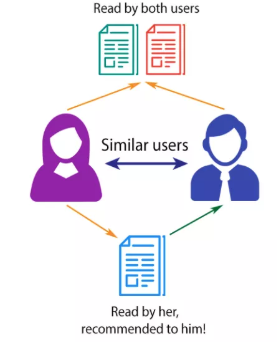
\includegraphics[width=7cm]{img/colaborative filtering.png}}%
           {\scriptsize%
            Zdroj: \url{https://towardsdatascience.com/the-remarkable-world-of-recommender-systems-bff4b9cbe6a7}}
  \caption{Collaborative filtering}
  
  \label{collaborativeFiltering}
\end{figure}

Existujú dva prístupy pri používaní tejto techniky:
\begin{enumerate}
	{\bf \item Memory-based metódy} niekedy označované aj ako neighbourhood-based collaborative filtering metódy, sú metódy v ktorých hodnotenia položiek používateľom, sú predpovedané na základe jeho susedov. Týchto susedov môžeme ďalej definovať dvoma spôsobmi:
\begin{itemize}[leftmargin=*]
	{\bf \item User-based}\newline	
Predpovedá hodnotenie používateľa \textit{u} položky \textit{i}, použitím hodnotení \textit{i} od iných používateľov, ktorí sú čo najviac podobní \textit{u}. Inak povedané snaží sa nájsť iných podobných používateľov (susedov) a odporúčať používateľovi \textit{u} produkty ktoré sa páčia im.
	{\bf \item Item-based} \newline
Zatiaľ čo pri user-based metóde sa pri predpovedaní hodnotenia spoliehajú na názor rovnako zmýšľajúcich používateľov, item-based prístupy sa zameriavajú na hodnotenie udelené podobným položkám. Túto myšlienku môžeme sformalizovať nasledovne. Predpoveď hodnotenia používateľa \textit{u} položky \textit{i} môžeme získať ako vážený priemer hodnotení \textit{u} iných položiek, ktoré sú čo najviac podobné \textit{i}.
\end{itemize}
	{\bf \item Model-based methods} využívajú metódy strojového učenia na tvorbu predpovedí, pričom tento problém považujú ako normálny problém strojového učenia. Využívajú sa techniky ako \acrshort{pca}, \acrshort{svd}, faktorizácia matíc, clusterin či neurónové siete. \\
\end{enumerate}


Collaborative filtering, hlavne typ neighbourhood-based, prináša jeho používaním zaujímavé výhody. Spomeňme pár z nich:
\begin{itemize}[leftmargin=*]
	{\bf \item Jednoduchosť} - Neighborhood-based metódy sú intuitívne a ich implementácia je relatívne jednoduchá. V ich najjednoduchšej podobe vyžaduje vyladenie iba jeden parameter (počet susedov použitých v predikcii).
	{\bf \item Účinnosť} - Jednou zo silných stránok, je ich efektívnosť. Na rozdiel od väčšiny model-based systémov nevyžadujú nákladné tréningové fázy, ktoré je potrebné vo veľkých komerčných aplikáciách vykonávať v častých intervaloch. Zatiaľ čo fáza odporúčaní je zvyčajne nákladnejšia ako pre model-based techniky, najbližších susedov je možné vopred vypočítať offline, čo poskytuje takmer okamžité odporúčania. Ukladanie najbližších susedov navyše vyžaduje veľmi málo pamäte, čo robí tento prístup škálovateľným na aplikácie s miliónmi používateľov.
	{\bf \item Zdôvodnenie odporúčaní} - Takéto metódy tiež poskytujú stručné a intuitívne odôvodnenie vypočítaných predikcií. Napríklad v item-based odporúčaní, zoznam susedových položiek, ako aj hodnotenie, ktoré používateľ týmto položkám dal, sa môžu používateľovi zobraziť ako odôvodnenie odporúčania. To môže pomôcť používateľovi lepšie pochopiť odporúčanie resp. jeho relevantnosť a môže slúžiť ako základ pre interaktívny systém, kde si môžu používatelia vybrať susedov, ktorým by sa mala venovať väčšia dôležitosť.
\end{itemize}


Hlavnou nevýhodou týchto systémov je tzv. "cold start problem", čo znamená, že je takmer nemožné niečo odporučiť novému používateľovi, alebo odporúčať novú položku používateľom, pokiaľ či už používateľ alebo položka nemajú žiadne interakcie. Navyše mnoho používateľov a položiek má príliš málo interakcií nato, aby algoritmus s nimi vedel na začiatku efektívne pracovať. Riešenia tohto problému bývajú, že novým používateľom sa odporúčajú náhodné položky a nové položky sa odporúčajú náhodným používateľom (tzv. "random strategy"). Často sa používa aj odporúčanie populárnych položiek novým používateľom a odporúčanie nových položiek najviac aktívnym používateľom (tzv. "maximum expectation strategy"). V skorej fáze "života" používateľa alebo položky, sa môže použiť iná metóda ako collaborative filtering. \\
	
 
\subsubsection{Content based filtering}
\label{sec:contentbased}
Táto technika zahŕňa odporúčanie položiek na základe ich samotných vlastností. Odporúčania sú tu vytvárané na základe predchádzajúcich interakcií jednotlivých používateľov s položkami. Systém pracujúci touto metódou, sa snaží hľadať podobnosti medzi položkami, s ktorými mal používateľ v minulosti pozitívnu interakciu (t.j. kúpil si daný produkt, ohodnotil kladne daný film, pridal skladbu do obľúbených atď.). Napríklad ak používateľ pozitívne ohodnotí film zo žánru komédia, systém z toho môže vyčítať, že do jeho preferencií patrí aj tento žáner a teda mu odporúčať komediálne filmy. Princíp fungovania je znázornený aj na \hyperref[contentFiltering]{obrázku \ref{contentFiltering}}.

Nato aby táto technika správne fungovala, si systém musí vytvoriť pri danom používateľovi akýsi model, resp. profil, ktorý reprezentuje používateľove preferencie, ktoré získa na základe vlastností pozitívne hodnotených položiek. Proces tvorby odporúčaní potom pozostáva z hľadania zhody medzi atribútmi profilu a atribútmi prehľadávaných položiek. Položky, ktoré sú odporúčané používateľovi, sú teda reprezentované, ako súbor vlastností tiež nazývaných aj atribúty. Napríklad pri odporúčaní filmov, vlastnosti, ktoré opisujú film sú herci, režiséry, žánre, hodnotenie filmu atď.\\\\
\begin{figure}[!htbp]
  \centering  
  \def\stackalignment{c}
	\stackunder{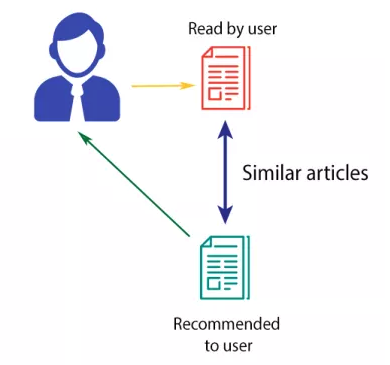
\includegraphics[width=7cm]{img/content-based-filtering.png}}%
           {\scriptsize%
            Zdroj: \url{https://towardsdatascience.com/the-remarkable-world-of-recommender-systems-bff4b9cbe6a7}}
  \caption{Content based filtering}
  
  \label{contentFiltering}
\end{figure}

Na získavanie feedbacku od používateľa sa používajú dva spôsoby: 
\begin{itemize}[leftmargin=*]
	{\bf \item like/dislike} - položky sú jednoducho klasifikované, buď ako relevantné, alebo irelevantné (binárne hodnotenie)  
	{\bf \item rating} - používa sa diskrétna numerická stupnica (numerické hodnotenie) \\
\end{itemize}

{\bf \large Výhody content based filteringu} \newline
	Implementácia content based odporúčaní má niekoľko výhod oproti ostatným technikám. 

\begin{itemize}[leftmargin=*]
	{\bf \item Nezávislosť od používateľov} - Tá je dosiahnutá vďaka tomu, že profil používateľa, na základe ktorého sa hľadajú zhody s položkami, je vytvorený len z hodnotení položiek daným používateľom. Naproti tomu, napríklad technika collaborative filtering potrebuje hodnotenia aj od iných používateľov, čo môže byť problém pri aplikáciách, kde nieje dostatočne veľký počet používateľov.
	{\bf \item Transparentnosť} - Zistiť ako systém funguje, je možné pomocou atribútov, ktoré model zohladňuje pri vytváraní profilu. To vie pomôcť pri porozumení, prečo sa konkrétna položka objavila v zozname odporúčaných. Collaborative filtering systémy sa podstatne ťažšie analyzujú, keďže jediné vysvetlenie prečo je položka odporúčaná je, že neznámy používateľ, s podobnými preferenciami, pozitívne hodnotil danú položku.
	{\bf \item Nová položka} - V content based metóde je možné odporúčať aj novú položku, ktorá nebola ešte hodnotená žiadnym používateľom. Vďaka tomu netrpí tzv. "frist-rater" problémom, ktorý postihuje collaborative filtering. Ten sa pri tvorbe odporúčaní spolieha na používateľské preferencie. To spôsobuje, že pokiaľ nová položka nebude hodnotená dostatočným počtom používateľov, systém nebude schopný ju odporúčať. \\
\end{itemize}


{\bf \large Nevýhody content based filteringu} \newline
	Napriek spomenutým výhodám, použitie tejto techniky prináša aj isté obmedzenia. 

\begin{itemize}[leftmargin=*]
	{\bf \item Nový používateľ} - Nato aby systém dokázal naozaj dobre porozumieť používateľovým preferenciám a vytváral presné odporúčania, je nevyhnutné mať zozbieraných dostatok hodnotení. Preto pri nových používateľoch, ktorí majú zo začiatku málo hodnotení, systém väčšinou neprináša spolahlivé odporúčania. 
	{\bf \item Over-specialization} - Známy problém, kedy systém odporúča položky, ktoré sú počas procesu zhody s používateľovým profilom označené ako užitočné. Tie však často bývajú podobné, ako položky, ktoré už hodnotil. Tento problém je často označovaný aj ako "serendipity problem", čím sa zdôrazňuje tendencia systému produkovať odporúčania, ktoré sa často podobajú a neobmieňajú. Napríklad ak používateľ pozitívne hodnotil filmy od režiséra Stanleyho Kubricka, v odporúčaniach mu môžu prevažovať filmy tohto typu. \\
	
\end{itemize}


\subsection{Mobilné aplikácie}
Mobilná aplikácia je softvérová aplikácia vytvorená špecificky pre mobilné zariadenia ako napríklad smartfóny, tablety alebo inteligentné hodinky. Pôvodne boli aplikácie vytvárané výrobcami mobilných operačných systémov, ktorí potrebovali pre používateľov zjednodušiť používanie základných funkcií smartfónu, ako napríklad prezeranie emailov, správ o počasí, prácu s kalendárom, fotenie fotografií atď. Avšak, vďaka rýchlemu vývinu samotných smartfónov a ich operačných systémov, začal rásť dopyt aj po aplikáciách zameraných na iné oblasti. V dnešnej dobe sú najpopulárnejšie rôzne herné aplikácie, navigačné aplikácie, aplikácie na online komunikáciu, hudobné aplikácie a mnohé iné. V posledných rokoch si používanie smartfónu bez spomenutých aplikácií ani nevieme predstaviť a stali sa ich neoddeliteľnou súčasťou. Aplikácie sa väčšinou sťahujú z distribučných platforiem, ktoré sú prevádzkované vlastníkom daného operačného systému, na ktorý je aplikácia určená. Spomeniem dva najväčšie a to App Store patriaci pod operačný systém iOS a Google Play Store patriaci pod Android. Na oboch platformách vieme nájsť veľké množstvo aplikácií všemožného zamerania, pričom každým dňom pribúdajú ďalšie. Niektoré sú bezplatné, iné spoplatnené tvorcom, pričom zárobok z nej sa delí medzi tvorcu aplikácie a distribučnú platformu. \\
\subsubsection{Typy mobilných aplikácií}
\label{sec:typy aplikacii}
Vo všeobecnosti sa mobilné aplikácie delia na 3 základné kategórie. Natívne aplikácie, webové aplikácie a hybridné aplikácie. Dnes však už je pri niektorých frameworkoch ťažké určiť, do ktorej kategórie presne patria, keďže kombinujú vlastnosti viacerých z nich, preto sme spomenuli aj tzv. cross-platform aplikácie.
\begin{itemize}[leftmargin=*]
{\bf \item Natívne aplikácie} - sú vytvorené výlučne pre špecifický mobilný operačný systém tj. napríklad natívne Android aplikácie alebo natívne iOS aplikácie. Kvôli špecifickému zameraniu na jeden operačný systém nie je možné aplikácie kombinovať na rôznych platformách. Napríklad Blackberry aplikácia nie je spustiteľná na Androide, Windows Phone aplikáciu zase nespustíme na iOS. Teda všeobecne povedané, mobilnú aplikáciu nainštalujete a spustíte len na operačnom systéme, pre ktorý je vytvorená. Inštalujú sa priamo do mobilného zariadenia, potrebné dáta sú väčšinou uložené priamo v internom úložisku zariadenia. \\

{\bf Používané technológie:} Na vývoj natívnych aplikácií sa používajú viaceré programovacie jazyky podľa toho, pre aký OS majú byť určené. Medzi najpoužívanejšie patria Java a Kotlin pre Android, Swift a Objective-C pre iOS. \\

{\bf Výhody:} Vďaka tomu, že sú zamerané na jednu platformu, vedia byť z hľadiska výkonu rýchlejšie a stabilnejšie. Hardvér zariadenia vedia využívať efektívnejšie. Sú schopné priamo pristupovať k všetkým funkciám zariadenia, vďaka čomu vedia využiť širokú ponuku možností, ktoré dané zariadenie ponúka ako napríklad fotoaparát, kontakty zariadenia, bluetooth, NFC či dokonca samotnú polohu zariadenia (GPS). Veľkú obľubu im zabezpečuje aj to, že využívajú natívny \acrshort{ui}, čo prináša používateľom lepší \acrshort{ux}. Niektoré nevyžadujú na funkčnosť internetové pripojenie. \\
 
{\bf Nevýhody:}  Primárnym problémom je duplicita pri vývoji aplikácie, keďže je potrebné aplikáciu naprogramovať pre viaceré mobilné operačné systémy, čo priamoúmerne zvyšuje cenu nehovoriac o náročnosti údržby a aktualizácie kódu pri každej novej verzii. Menší komfort spôsobuje aj fakt, že ak používateľ nechce prísť o najnovšiu funkcionalitu a opravu chýb, mal by pri každej aktualizácií aplikáciu preinštalovať resp. si nainštalovať tzv. update. \\

{\bf \item Webové aplikácie} - správajú sa podobne ako natívne aplikácie, najpodstatnejší rozdiel je v tom, že sa k nim pristupuje pomocou webového prehliadača. Sú to v podstate responzívne webové stránky, ktoré sa prispôsobujú svojim vzhľadom zariadeniu na ktorom sú spustené. \\

{\bf Používané technológie:} Webové aplikácie sú vytvorené pomocou HTML, ktorého vzhľad je naštýlovaný pomocou CSS a extra funkčnosť väčšinou zabezpečuje JavaScript. \\

{\bf Výhody:} Keďže na svoje fungovanie využívajú webový prehliadač, v tomto prípade zaniká problém duplicity pri programovaní aplikácie na viaceré operačné systémy. Toto znižuje náročnosť či už na vývoj, alebo cenu. Navyše odpadá potreba sťahovania, inštalácie a aktualizovania čo znamená, že aplikácia nezaberie žiadny priestor v úložisku zariadenia.  \\
 
{\bf Nevýhody:}  Hlavná nevýhoda pramení už z názvu - webové aplikácie, z čoho vyplýva, že bez internetového pripojenia ich nieje možné využívať. Webový prehliadač vie tiež ovplyvniť \acrshort{ux}. Kým v jednom môže byť k dispozícií plná funkcionalita, môže sa stať, že na druhom už len obmedzená. Programátori sa tomu samozrejme snažia zabrániť a programovať aplikácie tak, aby boli plne funkčné na čo najväčšom množstve najviac používaných prehliadačov. Nevýhodou je tiež značne obmedzený prístup k pokročilejším funkciám zariadenia ako napríklad využívanie gest. \\
 
{\bf \item Hybridné aplikácie} - sú založené na princípe miešania prvkov natívnych a webových aplikácií. Jadro aplikácie je napísane pomocou webových technológií (HTML, CSS, JavaScript), pričom je spúšťané z natívnej aplikácie a jej vlastného zabudovaného prehliadača, ktorý je ale pre používateľa neviditeľný. Napríklad aplikácia pre iOS by na zobrazenie používala WKWebView objekt, zatiaľ čo v Androide by na vykonávanie rovnakej funkcie používala WebView objekt. Kód samotný, je potom vložený do kontajnera natívnej aplikácie s použitím frameworkov ako Apache Cordova (známy aj ako PhoneGap), alebo Ionic. Tieto frameworky navyše majú aj systém pluginov, ktorý umožňuje ľahko prekonať obmedzenia webových aplikácií a rozšíriť funkcionalitu nad rámec prehliadača. Aplikácia tak môže získať plnú kontrolu nad funkciami mobilného zariadenia, čo umožňuje napríklad použiť TouchID pri iOS ako možnosť prihlásenia sa do aplikácie.\\


{\bf Používané technológie:} Hybridné aplikácie používajú kombináciu webových technológií a natívnych API. Sú vyvinuté pomocou technológií ako Ionic, Apache Cordova, Swift, HTML5, CSS, a JavaScript.  \\

{\bf Výhody:} Kombinácia dobrého \acrshort{ux}, menšej náročnosti pri vývoji a prijateľná cena, sú často hlavné činitele v ktorých hybridné aplikácie predčia konkurenciu. Vďaka tomu, že je z veľkej časti použitý rovnaký zdrojový kód, nezávisle od mobilného operačného systému. Na vývoj je potrebných menej vývojárov (napr. nemusia byť zvlášť tímy vývojárov pre iOS a zvlášť pre Android).  \\
 
{\bf Nevýhody: }  Najväčším mínusom hybridných aplikácií je výkon. Keďže sa načítavajú v spomínanom WebView objekte podobnom webovému prehliadaču, sú vysoko závislé od jeho samotného výkonu keďže je zodpovedný za zobrazovanie \acrshort{ui} a beh kódu. Napriek tomu, že aplikácie vedia bežať na viacerých operačných systémoch, je vcelku náročné si túto vlastnosť udržať. Občas vďaka výdavkom na implementáciu cross platformingu, vie cena hybridnej aplikácie dosiahnuť ceny natívnych aplikácií. Všetko však záleží od požiadaviek a od toho, ako veľmi sa chceme priblížiť k danej natívnej aplikácií.\\


{\bf \item Cross platform aplikácie} - sú špeciálnym typom aplikácií, ktoré sú veľmi podobné hybridným, pričom ale ponúkajú aj vlastnosti natívnych aplikácií. Na ich vývoj sa používajú špeciálne frameworky, pričom kód je napísaný v bežných programovacích jazykoch ako C\# alebo JavaScript. Aplikácie využívajú komponenty daných frameworkov, ktoré sú potom kompilované do natívneho kódu pre konkrétnu platformu. \\


{\bf Používané technológie:} Využívajú sa hlavne frameworky ako Xamarin, React Native a Flutter.  \\

{\bf Výhody:} Veľmi podobné hybridným aplikáciám. Jeden zdrojový kód kompilovateľný do viacerých OS, natívny \acrshort{ui} a prijateľná cena vývoja. Oproti hybridným aplikáciám sú na tom lepšie čo sa týka výkonu, keďže nebežia vo WebView objekte.  \\
 
{\bf Nevýhody:} Vývojári sú pri vývoji značne obmedzený ponukou komponentov, ktoré daný framework poskytuje. Z hľadiska výkonu, sú na tom čisto natívne aplikácie stále o niečo lepšie. Pri jednoduchých aplikáciách to však nie je badateľné.  \\
\end{itemize}

\subsubsection{Prečo sme si vybrali React Native?}
Pri rozhodovaní o hlavnej technológií na vývoj našej aplikácie, sme uvažovali nad dvoma možnosťami. Porovnávali sme Android Studio, ktorého programovacím jazykom je Java a vytvorili by sme teda čisto natívnu aplikáciu pre Android a cross platformový framework React Native, ktorý využíva JavaScript. Po zvážení náročnosti jednotlivých riešení, ich výhod a nevýhod, potenciálu do budúcnosti a subjektívnych sympatií, sme vybrali React Native. Detailnejšie sa mu budeme venovať \hyperref[sec:React Native]{v nasledujúcej kapitole.} \\


\subsection{React Native}
\label{sec:React Native}

React Native je cross-platformový framework na vývoj mobilných aplikácií, ktorý je postavený na populárnom webovom frameworku React. Rovnako ako React, aj React Native je open-source projekt udržiavaný prevažne vývojármi Facebooku a Instagramu. Potom ako sa v roku 2012 Mark Zuckerberg vyjadril, že používanie veľkého množstva HTML5 v mobilnej aplikácií Facebooku považuje za chybu. Vzhľadom nato, že výsledkom bola nestabilita aplikácie a pomalé načítavanie dát, sa Facebook rozhodol, že ich prioritou bude zlepšiť \acrshort{ux} ich mobilnej aplikácie. React na ktorom bol neskôr v roku 2015 postavený React Native, vytvoril Jordan Walke, softvérový inžinier Facebooku. Jeho prvý prototyp, ktorý bol inšpirovaný XHP (rozšírenie PHP ktoré umožňuje vytvárať upravené HTML elementy) sa nazýval FaxJS. Použitý bol prvýkrát v roku 2011 vo Facebookovom news feede a neskôr v roku 2012 na Instagrame. React Native bol ohlásený v roku 2015 na konferencii Facebooku a prvá verzia vyšla 26. marca toho roku. Od vtedy zaznamenal tento framework nárast popularity naprieč celým spektrom vývojárov mobilných aplikácií a je čoraz častejšie používaný. Sú pomocou neho vytvorené viaceré známe mobilné aplikácie ako Facebook, Instagram, Skype, Airbnb, Bloomberg, SoundCloud a mnohé iné. \\
\subsubsection{Princíp fungovania}
Pri vytváraní aplikácií pomocou React Native, je všetka logika, volania \acrshort{api} a management stavov v JavaScripte. V porovnaní s inými hybridnými frameworkami, aplikácia vytvorená v React Native nebeží vo WebView, ale používa tzv. komponenty ktorých logika a štýlovanie je napísané priamo v kóde, ale vyrendrované sú konkrétne do natívnej podoby podľa platformy. Vďaka tomu je zaručené vysoké percento recyklovania kódu (cca. medzi 85 - 99 \%), pričom \acrshort{ui} je prispôsobené konkrétnej platforme. V prípade, ak je to potrebné, React Native umožňuje písať kód, logiku a štýlovanie špecificky pre konkrétnu platformu. \\
\subsubsection{Bridge}
React Native aplikácia je zložená z dvoch častí, JavaScript kódu a natívneho kódu. Z technologického hľadiska je zaujímavé, že natívny kód je napísaný diametrálne odlišnými jazykmi. Pri iOS sa napríklad používa Objective-C alebo Swift, pri Androide Java či Kotlin. Bridge je koncept, ktorý umožňuje a zabezpečuje komunikáciu medzi týmito dvoma časťami. Je jedným z najdôležitejších princípov, bez ktorého by si natívny kód a JavaScript kód nevedeli medzi sebou vymieňať žiadne informácie. 
%\begin{figure}
%  \centering
%  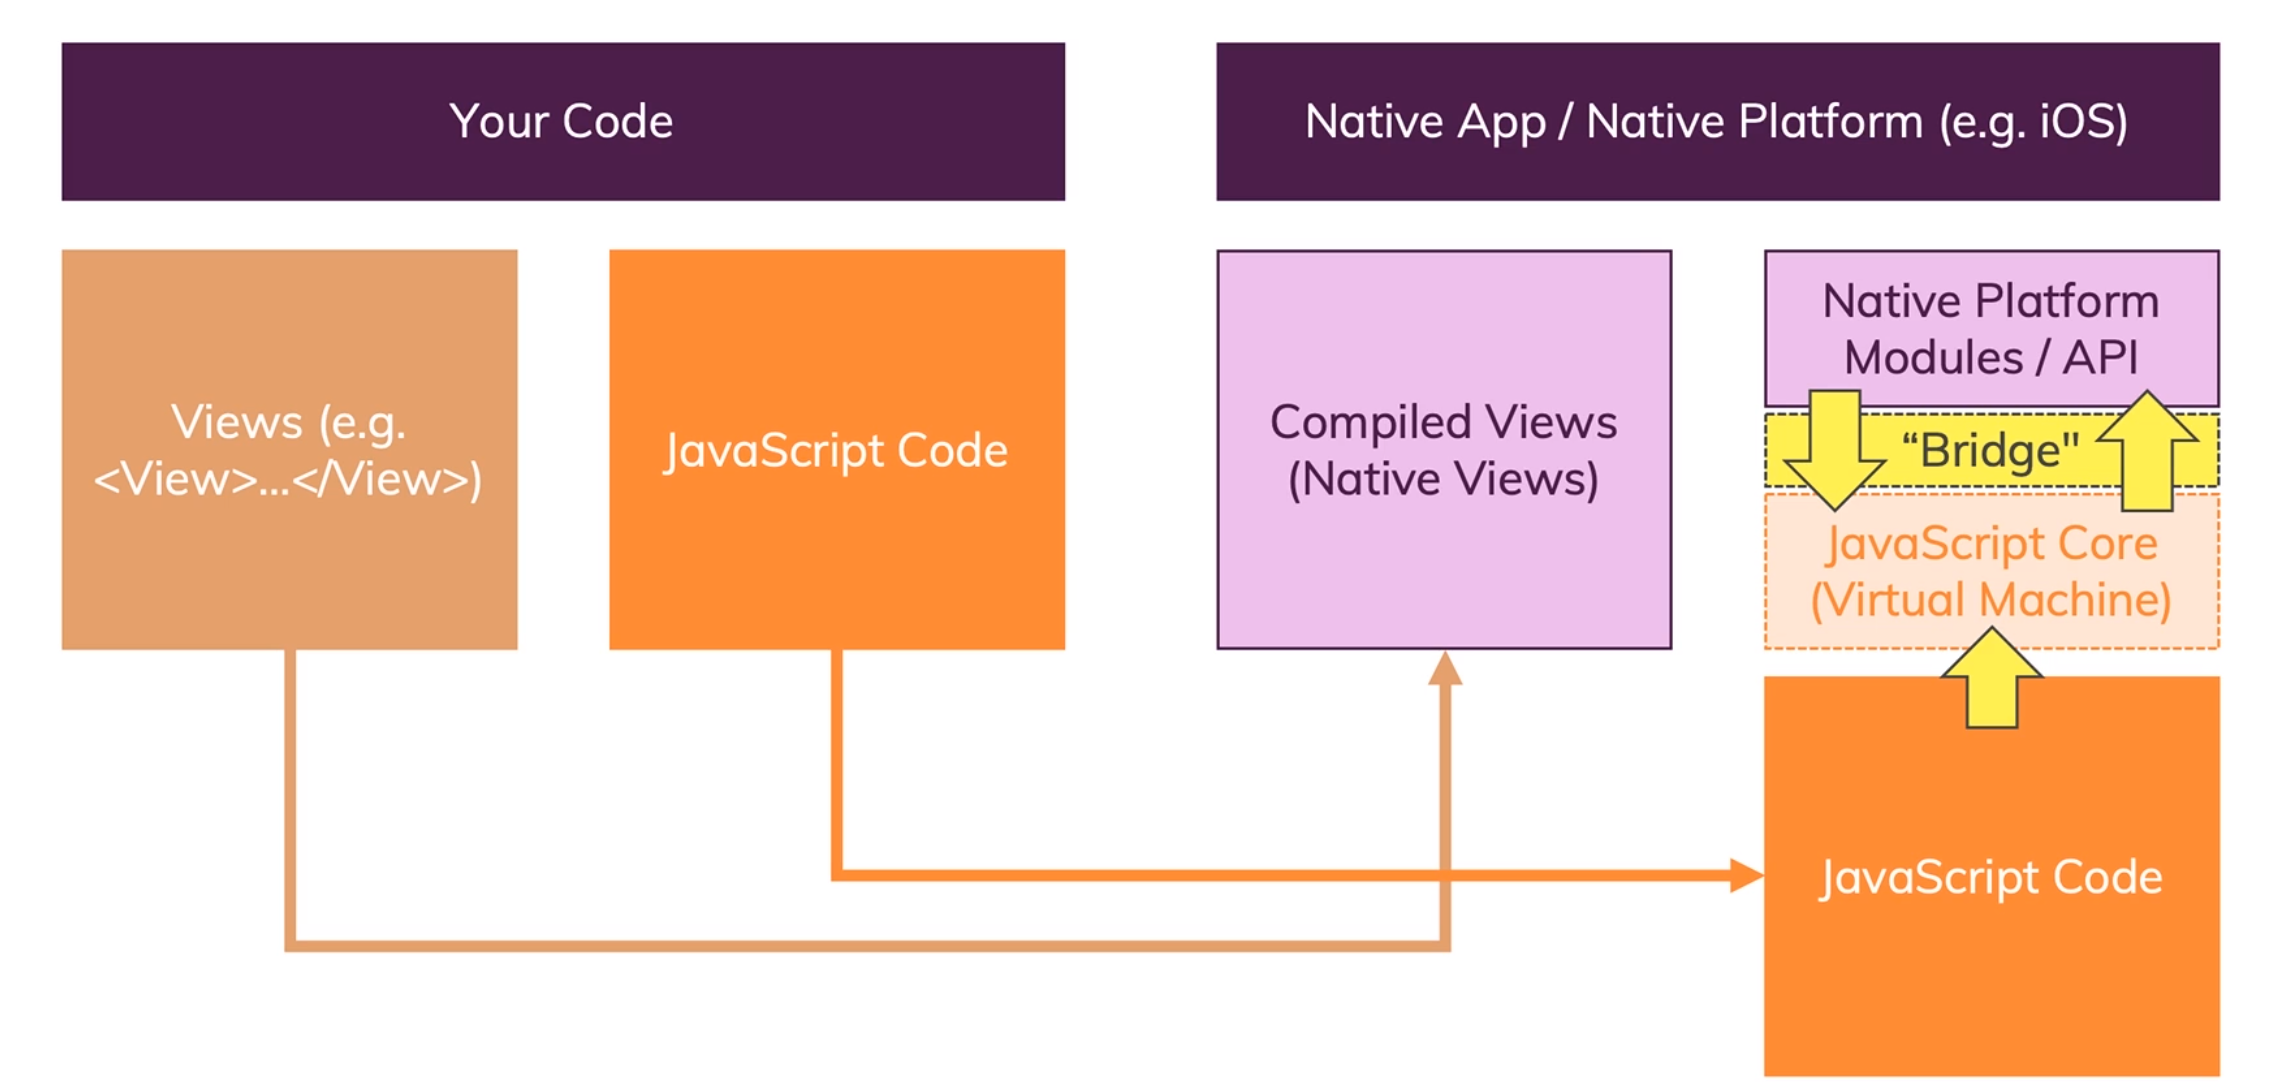
\includegraphics[width=15cm]{img/rn-working.png}
%  \caption{Ukážka fungovania React Native aplikácie}
%  \label{nativeappeg}
%\end{figure}	
\begin{figure}[!htbp]
  \centering  
  \def\stackalignment{c}
	\stackunder{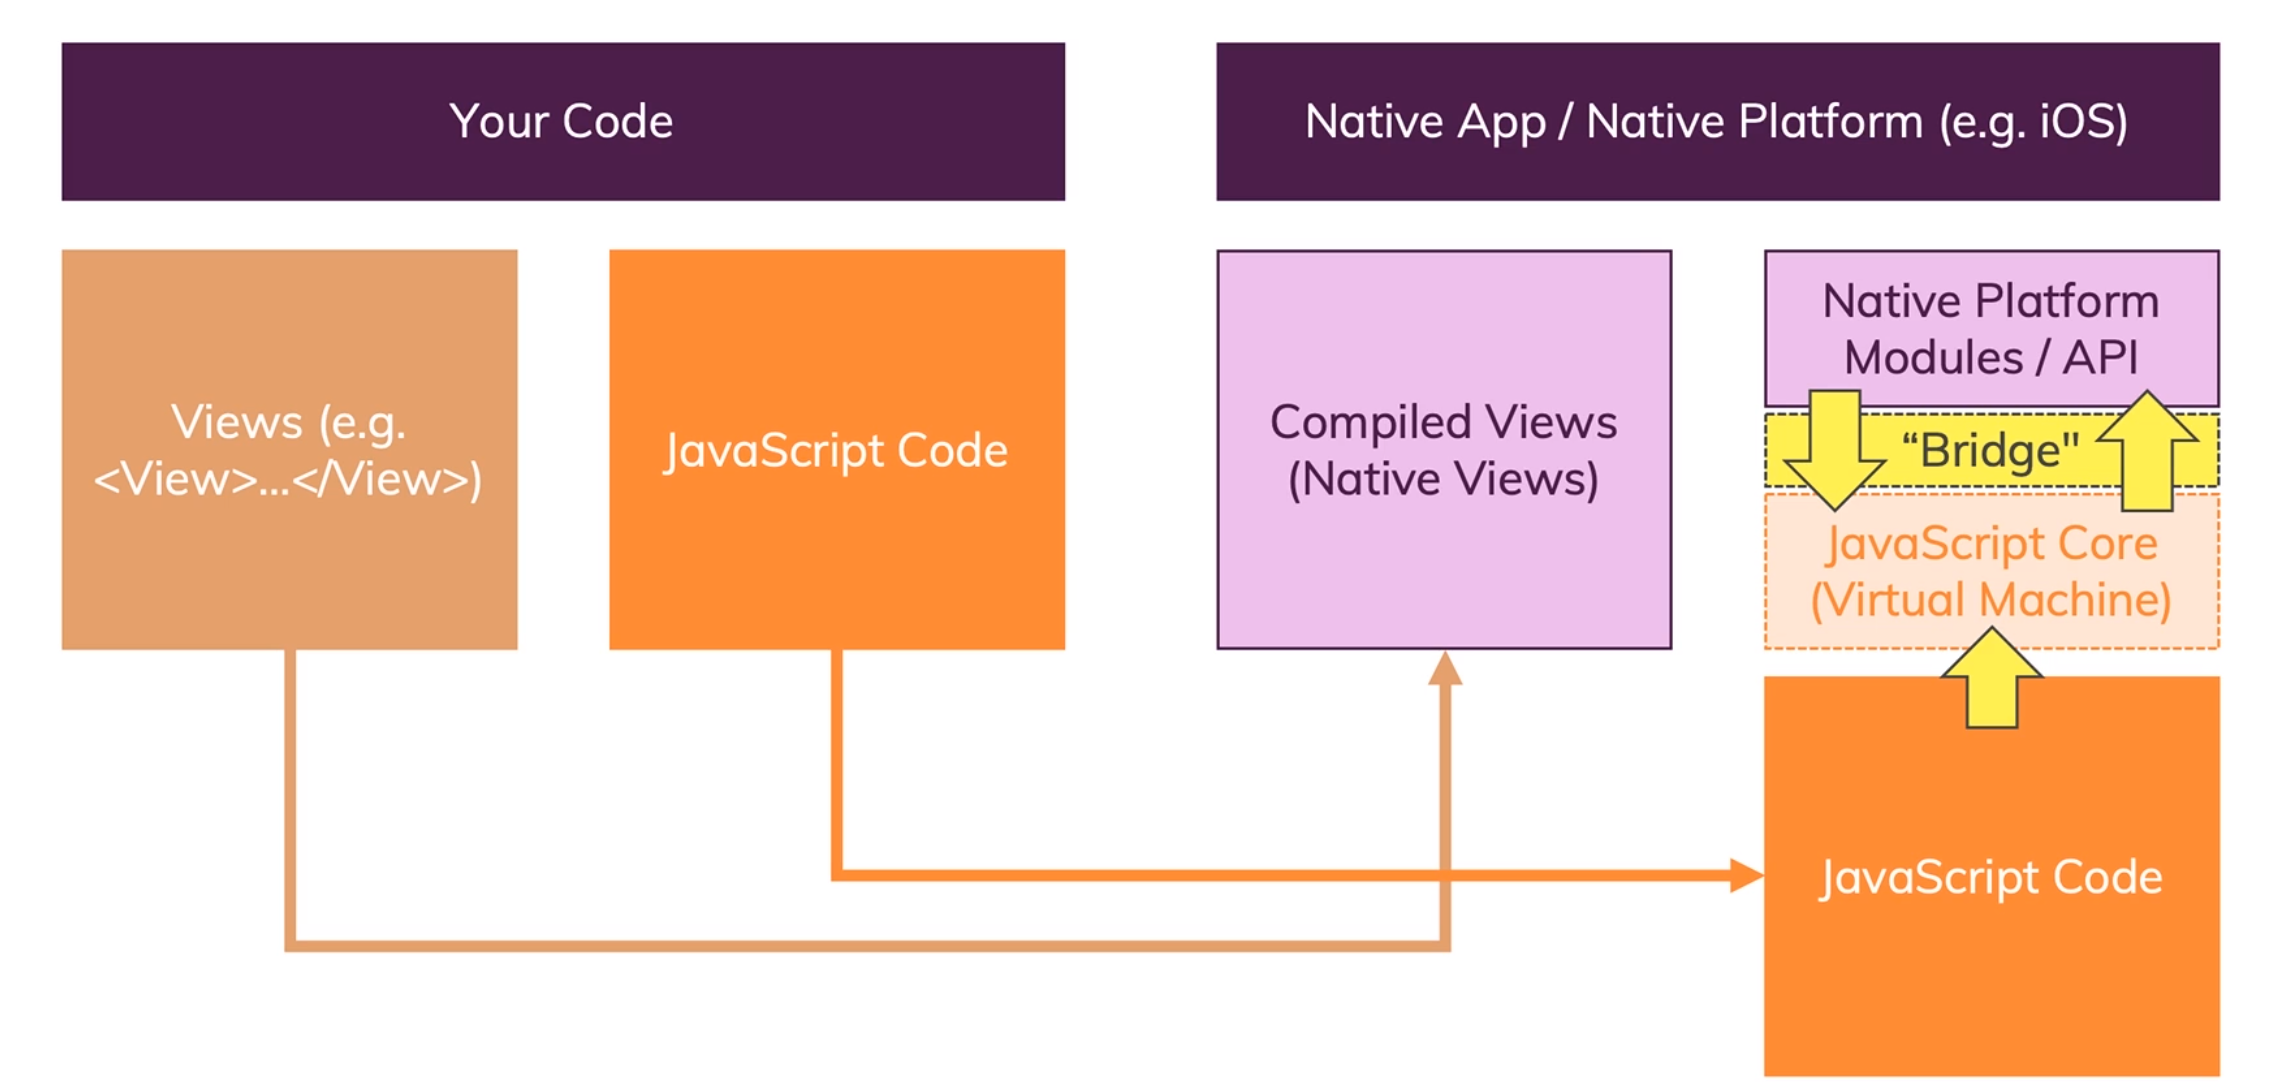
\includegraphics[width=15cm]{img/rn-working.png}}%
           {\scriptsize%
            Zdroj: \url{https://www.udemy.com/course/react-native-the-practical-guide/}}
	\caption{Ukážka fungovania React Native aplikácie}  
  \label{reactAppExplained}
\end{figure}
\subsubsection{Virtual DOM (Document Object Model)}
Ďalším dôležitým koncepotom v React Native, je tzv. Virtual DOM. Predtým, ako si vysvetlíme pracovanie s Virtual DOM v React Native, sa nato najprv pozrieme z pohľadu Reactu. DOM je vo všeobecnosti skratka pre Document Object Model (inak nazývaný aj real DOM), čo je programové rozhranie pre HTML a XML dokumenty. DOM reprezentuje dokument ako skupinu uzlov (tzv. "nodes") a objektov. To umožňuje jazykom ako napríklad JavaScript modifikovať dané uzly a tým aj celý dokument. DOM je reprezentovaný ako dátovy strom, vďaka čomu je každá zmena rýchla. Avšak po tejto zmene, zmenené elementy a ich potomkovia musia byť nanovo vyrendrované aby nastal aj priamo update UI danej aplikácie. Proces rendrovania je to, čo spôsobuje nezanedbateľné spomalenie výkonu, ktoré je navyše priamo úmerné so zväčšujúcim sa počtom UI komponentov, ktoré treba nanovo vyrendrovať.

Tu prichádza na scénu Virtual DOM a dosahuje podstatne lepšie výkonostné výsledky ako real DOM. Virtual DOM je iba virtuálne znázornenie DOM. Vždy, keď sa zmení stav aplikácie, namiesto real DOM sa aktualizuje virtual DOM. Keď je do UI pridaný nový element, vytvorí sa virtual DOM (reprezentovaný ako strom). Akonáhle sa zmení stav ktoréhokoľvek elementu, vytvorí sa nový virtual DOM, prebehne proces porovnania (nazývaný "diffing") aktuálnej verzie a prechádzajúcej verzie vritual DOM. Potom sa vypočíta najlepší možný spôsob ako tieto zmeny premietnuť do real DOM. Akonáhle React vie, ktoré elementy vo virtual DOM boli zmenené, zaktualizuje len dané elementy v real DOM. Vďaka tomu je výkon neporovnateľne lepší v porovnaní s priamou manipuláciou s DOM.

\begin{figure}[!htbp]
  \centering  
  \def\stackalignment{c}
	\stackunder{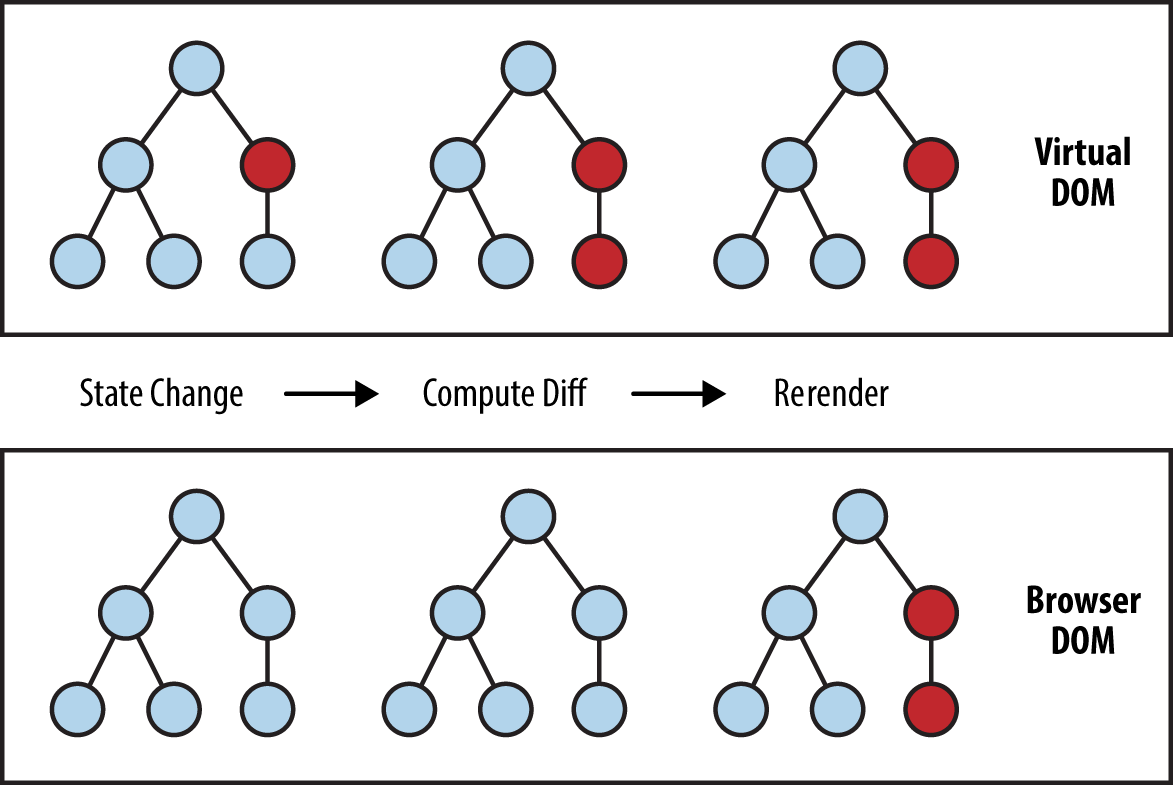
\includegraphics[width=12cm]{img/dom.png}}%
           {\scriptsize%
            Zdroj: \url{https://programmingwithmosh.com/react/react-virtual-dom-explained/}}
	\caption{Virtual DOM vs. real DOM}  
  \label{domImg}
\end{figure}
Na \hyperref[domImg]{obrázku \ref{domImg}} vidíme červené kruhy, ktoré znázorňujú zmenené uzly. Tieto uzly reprezentujú konkrétne UI elementy, ktorých stav sa zmenil. Následne je vypočítaný rozdiel medzi aktuálnou a predchádzajúcou verziou virtual DOM stromu, pričom celý podstrom rodiča je nanovo prerendrovaný a tým poskytne aktualizáciu UI. Aktualizácie real DOM sa posielajú hromadne, namiesto odosielania aktualizácií pre každú jednu zmenu stavu.

Spôsob akým virtual DOM využíva samotný React Native je vo veľkej miere podobný. Hlavnou odlišnosťou je, že sa namiesto webových komponentov rendrujú natívne komponenty, tým pádom sa nepoužívajú webové technológie. \\

\subsubsection{Základné komponenty}
Kľúčovým prvkom každej React Native aplikácie sú komponenty. Každý komponent má inú úlohu, no dokopy tvoria celok - samotnú aplikáciu. Z hľadiska koncepcie môžeme povedať, že komponenty sú podobné JavaScript funkciám. Vedia príjímať vstupy (nazývane ``props''), s ktorými potom umožňujú pracovať vo vnútri komponentu a vracajú elementy ktoré popisujú čo sa má zobraziť na obrazovke. V React Native existujú dva hlavné typy komponentov, ktoré tvoria aplikáciu. Sú štruktúrované rovnako, ako v bežnej webovej aplikácii vytvorenej pomocou Reactu.
\begin{itemize}[leftmargin=*]
{\bf \item Class komponenty} \newline
Sú to triedy rozširujúce základnú triedu z Reactu s názvom Component. Majú prístup k lifecycle metódam Reactu ako napríklad render či state/props funkcionalite od rodičovskej triedy. V súčasnosti sú menej používané kvôli tomu, že sú komplikovanejšie ako functional komponenty. Aj keď stále existujú prípady, v ktorých je ich syntax potrebná, vo všeobecnosti sa pri vytváraní nového komponentu viac používa syntax functional kompononetu. Vo \hyperref[classComponent]{výpise \ref{classComponent}} máme úvedený aj jednoduchý príklad class komponentu.  \\

\begin{lstlisting}[  caption={Príklad class komponentu}, label={classComponent} ]
import React, { Component } from 'react';
import { Text } from 'react-native';

class Cat extends Component {
  render() {
    return (
      <Text>This is class component!</Text>
    );
  }
}

export default Cat;
\end{lstlisting}
{\bf \item Functional komponenty} \newline
Sú najjednoduchší spôsob vytvorenia komponentu. Ich deklarácia je v podstate rovnaká ako pri obyčajnej JavaScript funkcii. V minulosti sa za ich nevýhodu oproti class komponentom považovalo to, že neumožňovali správu stavov (states) a nemali prístup k lifecycle metódam ktoré React Native poskytuje. To sa zmenilo až po vydaní verzie 16.8.0 v roku 2019, v ktorej vývojári pridali Hooks, čím tento problém zanikol. Odvtedy sa ich popularita ešte zvýšila a stali sa novým štandartom. Na \hyperref[funcComponent]{výpise \ref{funcComponent}} môžeme vidieť, že je jednoduchšie ich udržiavať ``light weight'' a kód je pri nich čitateľnejší, ako pri class komponentoch. \\

\begin{lstlisting}[caption={Príklad function komponentu}, label={funcComponent}]
import React from 'react';
import { Text } from 'react-native';

const Cat = () => {
  return (
    <Text>This is functional component!</Text>
  );
}

export default Cat;
\end{lstlisting}

\end{itemize}

React Native navyše poskytuje aj sadu predpripravených hotových natívnych komponentov, ktoré sa dajú veľmi jednoducho použiť pri programovaní aplikácie. Patria medzi ne napríklad View, Text, Button, Image, či TextInput. \\

\subsubsection{Props a state}
Props a State sú dva typy dát, pomocou ktorých vieme pracovať s komponentami.
\begin{itemize}[leftmargin=*]
{\bf \item Props} \newline
Props (z anglického slova ``properties'') je obdoba argumentov pri klasických funkciách v JavaScripte alebo atribútov pri HTML. Komponenty prijímajú props od rodičovského komponentu. Ich dôležitou vlastnosťou je, že sú tzv. ``immutable'' tj. nemenné vo vnútri komponentu. V Reacte a v React Native smerujú dáta jedným smerom - od rodičovských komponentov k detským. Celý koncept props je založený natom, že si viete vytvoriť jeden komponent, ktorý je možné použiť na viacerých miestach v aplikácii. Rodičovské komponenty potom vedia zavolať váš vytvorený komponent, pričom na rôznych miestach vie mať rozličné props. Props v zásade pomáhajú písať znovu použiteľný kód.
{\bf \item State} \newline
State pracuje odlišne v porovnaní s props. Je to interná vlastnosť komponentu, ktorá pomáha v rámci komponentu sledovať určité informácie. Použitím ``setState'' sa daný komponent aj jeho detské komponenty nanovo vyrendrujú, vďaka čomu sa nemusí programátor zaoberať implementáciou event handlerov ako v iných jazykoch. State sa používa v situáciách, keď sa menia dáta v rámci komponentu. Dobrým príkladom je napríklad interakcia používateľa s komponentom, pri klikntí na tlačidlo alebo zaškrtnutí checkboxu. Napríklad pri vypĺňaní formuláru má každý z textových inputov svoj vlastný state. Ak vyplníte daný input, automaticky sa mení jeho state, čo spôsobuje prerendrovanie celého komponentu a všetkých jeho detskych komponentov. \\
\end{itemize} 
\subsubsection{Hooks}
Hooks boli predstavené vo verzii 16.8.0 v roku 2019. Ich hlavnou úlohou je umožniť používať state a lifecycle metódy vo functional komponentoch, čo predtým bolo možné iba vytvorením class komponentov (v nich Hooks nie sú použiteľné). Ich uvedenie výrazne zvýhodnilo používanie functional komponentov oproti class komponentom. Tak isto ako pri komponentoch, aj tu React Native umožňuje využiť predpripravené Hooks priamo od vývojárov. Najčastejšie používané sú useEffect a useState. V prípade potreby je možné si vytvoriť aj vlastný hook tak, aby spĺňal požadovanú funkcionalitu. \\
\subsection{Expo alebo React Native CLI ?}
Predtým ako sa programátor pustí do vývoja aplikácie pomocou React Native, ho čaká rozhodnutie či použiť pomocný framework Expo, alebo vstavanú funkcionalitu React Native CLI. Nato aby sme mohli vytvorenú aplikáciu vôbec spustiť, potrebujeme jednu z týchto technológii. \\



\subsubsection{Expo}
Framework používaný pri vytváraní React Native aplikácií. Je to balík nástrojov a služieb vytvorených pre React Native, ktoré pomáhajú pri vývoji aplikácie. \newline

{\bf Výhody}
\begin{itemize}
{\item Nevyžaduje vedomosť programovania v natívnom kóde.}
{\item Nepoužíva Xcode alebo Android Studio.} 
{\item Najrýchlejší a najjednoduchší spôsob, ako vytvoriť natívne React Native aplikácie.}
{\item Uvolňuje OTA updates.} 
{\item Vstavaný prístup k natívnym APIs.}
\end{itemize}

{\bf Nevýhody}
\begin{itemize}
{\item Ďalšia vrstva abstrakcie.} 
{\item Neumožňuje zasahovať do natívneho kódu.}
{\item Niesu k dispozicií všetky iOS a Android APIs.} 
\end{itemize}
\bigskip

\subsubsection{React Native CLI}
Vstavaný nástroj v React Native, ktorý pomáha spustiť aplikáciu. \newline

{\bf Výhody}
\begin{itemize}
{\item Umožňuje zasahovať do natívneho kódu.} 
{\item Vieme pomocou neho pridávať natívne moduly (Objective C/Java).} 
\end{itemize}

{\bf Nevýhody}
\begin{itemize}
{\item Vývoj iOS aplikácie nie je možný na inom OS ako MacOS.} 
{\item Na vytvorenie projektu sa vyžaduje Android Studio alebo XCode.}
{\item Nastavenie projektu (vrátane konfigurácie) je pomerne komplikované a nepohodlné.} 
{\item Neposkytuje niektoré JavaScript APIs napr. notifikácie, je potrebné ich ručne doinštalovať.} \\
\end{itemize}

\subsubsection{Odôvodnenie výberu}
V našom prípade sme si vybrali pracovať s Expom, keďže práca s ním je jednoduchšia a priamočiarejšia a vzhľadom na typ a vlastnosti aplikácie, nám jeho funkcionalita plne postačuje. \\

\subsection{Node.js}
Node.js je open-source, cross-platformové, back-endové runtime prostredie JavaScriptu, ktoré beží na Chrome V8 JavaScript engine a vykonáva kód JavaScript mimo webového prehliadača. Tento engine prekladá JavaScriptový kód do rýchlejšieho strojového kódu. Strojový kód je nízkoúrovňový kód, ktorý počítač dokáže prečítať bez potreby ďalšej interpretácie. Vznik node.js bol logickým krokom po tom, ako vývojári JavaScriptu rozšírili použiteľnosť jazyka z čisto skriptovacieho, ktorý bolo možné používať a spúštať iba v prehliadači, na jazyk ktorý umožňuje vytvoriť samostatnú aplikáciu spustiteľnú aj mimo prehliadača. 

Nesporným prínosom node.js je, že využíva tzv. event-driven non-blocking I/O model, ktorý ho robí efektívnym. I/O alebo aj input/output, môže byť čokoľvek od čítania resp. zapisovania lokálnych súborov, až po vytváranie HTTP requestov na API. Non - blocking znamená, že napríklad pri requeste na vytiahnutie údajov dvoch používateľov z databázy, daný request neblokuje vykonávanie ďalšieho kódu počas čakania na odpoveď. Na \hyperref[nodejsImg]{ obrázku \ref{nodejsImg}} nižšie možeme vidieť porovnanie blocking (vľavo) a non blocking modelu (vpravo) na spomenutom príklade s databázou. \\

\begin{figure}[!htbp]
  \centering  
  \def\stackalignment{c}
	\stackunder{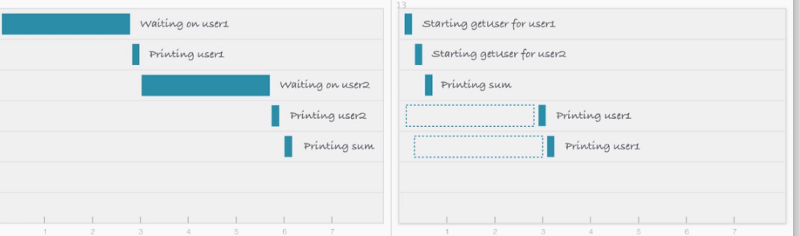
\includegraphics[width=16cm]{img/nodejs.png}}%
           {\scriptsize%
            Zdroj: \url{https://www.freecodecamp.org/news/what-exactly-is-node-js-ae36e97449f5/}}
	\caption{Porovnanie blocking a non-blocking modelu}  
  \label{nodejsImg}
\end{figure}

\subsubsection{Yarn}
Je package manager pre JavaScript, ktorý pomáha riadiť dodatočne doinštalované knižnice a rôzne iné dependencies v našom projekte. Keďže v súčasnej dobe sa pri programovaní využíva veľké množstvo knižníc a dependencies, aby sa zjednodušila práca programátora a nemusel istú funkcionalitu programovať nanovo, je odporúčané package manager používať. 

Node.js prichádza s predinštalovaným package managerom npm. Napriek tomu sme sa rozhodli použiť yarn, ktorý bol vytvorený Facebookom, tak isto ako React Native a preto práca s ním bola konzistentnejšia a bez väčších problémov na rozdiel od npm. \\
\subsubsection{Axios}
Axios je knižnica pre JavaScript, ktorá sa používa na vytváranie HTTP requestov z node.js alebo XMLHttpRequests z prehliadača. Podporuje aj ES6 promise API, pričom ešte viac uľahčuje celý proces okolo requestov tým, že ešte viac zlepšila dobre fungujúcu fetch() funckiu z JS a vylepšila error handling. \\


\subsection{TMDb}
The Movie Database (TMDb), je databáza filmov a TV seriálov, ktorá bola vytvorená v roku 2008 úzkou komunitou ľudí, ktorá sa neskôr postupne rozrástla. Dnes je TMDb používaná vyše 400 000 developermi a firmami. Úspech im prinisela hlavne ich dostupná API, ktorá je zadarmo a ponúka širokú škálu queries pomocou ktorých je možné získať podrobné informácie o filmových tituloch. Ich veľkou prednosťou je aj množstvo dostupných titulných plagátov k filmom vo vysokej kvalite. Jedinou jej nevýhodou je, že popularitou zatiaľ nedosahuje úroveň najväčšej databázy na svete IMDB a pri niektorých filmoch niesú ich hodnotenia kredibilné. \\

\subsection{Firebase}
Firebase je platforma vyvinutá spoločnosťou Google, ktorá pomáha vytvárať, zlepšovať a rozširovať funkcionalitu aplikácií. Obsahuje sadu nástrojov , ktoré pokrývajú veľkú časť služieb, ktoré by si vývojári museli inak sami naprogramovať. Patria sem napríklad analytika, autentifikácia používateľov, databázy, konfigurácia, ukladanie súborov, doručovanie push notifikácií a mnoho iného. Služby sú uložené v cloude a sú škálovateľné s malým resp. minimálnym úsilím zo strany vývojára. \\

\subsubsection{Firebase authentication}
\label{sec:firebaseauth}
Poskytuje backendové služby, jednoducho použiteľné SDK a predpripravené UI knižnice na autentifikáciu používateľov v aplikácii. Podporuje autentifikáciu pomocou hesla, telefónneho čísla, Googlu, Facebooku a Twitteru. Je úzko integrovaná s ostatnými službami Firebase a využíva  štandardy ako OAuth 2.0 a OpenID Connect, takže ju možno ľahko integrovať do vlastného backendu. Okrem autentifikácie umožňuje aj registráciu a správu zaregistrovaných používateľov. V našej aplikácií sme si zvolili použiť autentifikáciu pomocou hesla. \\

\subsubsection{Cloud firestore}
\label{sec:firestore}
Cloud Firestore je škálovateľná NoSQL cloudová databáza, pre vývoj mobilných a webových aplikácii. Udržuje dáta synchronizované medzi klientskými aplikáciami prostredníctvom listenerov v reálnom čase. Ponúka bezproblémovú integráciu s ostatnými produktami Firebase a Google Cloud vrátane cloudových funkcií. 

Vo firestore dátovom modeli \hyperref[firestore]{(pozri obr. \ref{firestore})}, sa dáta ukladajú do tzv. dokumentov, ktoré obsahujú polia (fields) namapované na konkrétne hodnoty. Tieto dokumenty sú ukladané do kolekcií, ktoré slúžia ako kontainer pre viacero dokumentov. Dokumenty podporujú mnoho rôznych dátových typov, od jednoduchých ako sú napríklad reťazce alebo čísla, až po komplexnejšie ako mapy, polia, alebo komplexné vnorené objekty. Vytvoriť komplexnú databázu umožňuje vytváranie subkolekcií v rámci dokumentu (tj. kolekcie osbahujú dokumenty, ktoré obsahujú kolekcie a tie obsahujú ďalšie dokumenty atď.). \cite{firestoredoc}
  
Friebase ponúka aj druhý typ databázy, Firebase Realtime Database, čo je tiež NoSQL cloudová databáza. Avšak, oproti firestore ponúka jednoduchší dátový model, v ktorom sa dáta ukladajú iba vo formáte JSON, čo je vhodné iba pri jednoduchšej dátovej štruktúre. Taktiež nepodporuje používanie zložitejších queries. Firestore bol teda v našom prípade lepšou voľbou v oboch prípadoch. \\

\begin{figure}[!htbp]
  \centering  
  \def\stackalignment{c}
	\stackunder{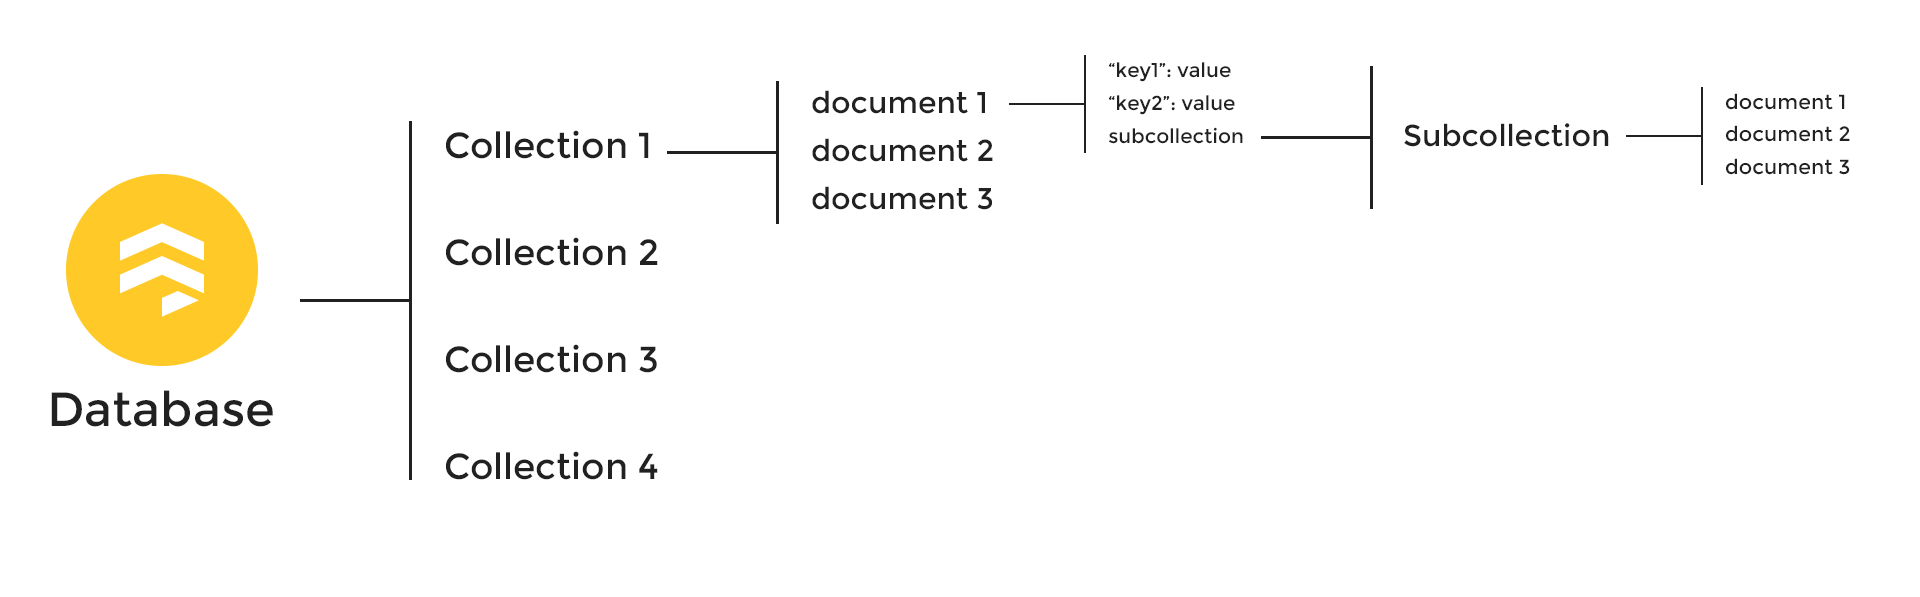
\includegraphics[width=15cm]{img/firestore.png}}%
           {\scriptsize%
            Zdroj: \url{https://waelyasmina.com/firebase-cloud-firestore-tutorial-web/}}
	\caption{Znázornenie dátového modelu Cloud Firestore}  
  \label{firestore}
\end{figure}




\section{Analytická a návrhová časť}
\subsection{Analýza problému}
V dnešnej dobe, kedy je ponuka produktov na trhuv veľmi veľká a pestrá, býva častým problémom používateľov nájsť práve tie produkty o ktoré majú reálne záujem a vyhovujú ich kritériám. Práve tento problém bol motiváciou pre vznik odporúčacích systémov \hyperref[sec:odporucacie systemy]{(kapitola 1.1)}, ktoré sa dnes vo veľkej miere využívajú. 

Jedným z prípadov, pri ktorom sa s daným problémom často stretávame, je výber filmového titulu. S príchodom streamovacích služieb ako Netflix, Amazon Prime, Hulu či HBO GO, vďaka ktorým sú dostupné milióny titulov, je veľmi náročné vybrať si tie, ktoré budú vyhovovať osobným preferenciám jednotlivca. Vačšina spoločností to vyriešila zavedením odporúčacích systémov a používaním rôznych rebríčkov popularity. To však vyriešilo iba situáciu, ak sa človek rozhodne pozerať film sám. Bežne sa však stáva, že ľudia chcú pozerať film vo dvojici a pri spoločnom výbere filmu strávia neprimerane veľa času prezeraním rôznych filmových databáz a rebríčkov filmov. 

To nám vnuklo myšlienku, na tému tejto bakalárksej práce s cieľom zjednodušiť výber filmu  prostredníctvom mobilnej aplikácie, založenej na odporúčacích systémoch.

\subsection{Existujúce riešenia problému}
Pri analýze súčasného stavu sme sa pozreli na existujúce riešenia, venujúce sa danej problematike. Je dôležité poznamenať, že v čase zadania práce nebola dostupná aplikácia, ktorá by obsahovala podobnú funkcionalitu a bola by dostupná na oba spomínané operačné systémy. 
\subsubsection{Android OS}
Na OS Android bola dostupná len 1 aplikácia vytvorená v roku 2019, avšak už dlhšie nepodporovaná vývojárom. Aplikácia s názvom MovieMatch má však viacero nevýhod oproti riešeniu, ktoré sme navrhli my. Základným prvkom tejto aplikácie je skupina, kým v žiadnej nie ste nemáte možnosť si prezerať a hodnotiť filmové tituly. Po nainštalovaní a spustení, vygeneruje aplikácia kód, ktorý treba poslať iným používateľom, aby sa mohli pripojiť do jeho skupiny. Tak isto sa používateľ vie pripojiť do inej skupiny pomocou kódu danej skupiny. Toto riešenie spôsobuje, že používateľ je zavislý od iných používateľov a bez nich je aplikácia nepoužiteľná.Nevýhodou tohto riešenia je aj spôsob implememtácie, vo forme webovej aplikácie, ktorá sa otvára priamo v prehliadači. To vzhľadom na súčasné štandardy vývoja mobilných aplikácií nie je najvhodnejšie riešenie a UI oproti natívnym a hybridným (resp. cross platformovým) aplikáciám pôsobí zastaralo. Detailnému porovnaniu typov mobilných aplikácií sme sa venovali v \hyperref[sec:typy aplikacii]{kapitole 1.2.}
\subsubsection{iOS}
V čase zadania tejto bakalárskej práce nebola podobná aplikácia bežiaca na operačnom systéme iOS k dispozicií. To sa neskôr zmenilo, keď v novembri 2020 vyšla aplikácia Movie Match. Funkcionalitou a vzhľadom je na tom omnoho lepšie ako spomínaná Android aplikácia. Z jej používania však nie je jasné, či pri generovaní filmov využíva nejaký druh odporúčacieho algoritmu, alebo generuje filmy každému používateľovi rovnako. To ma za následok, že  používateľ nenadobudne pocit, že sa aplikácia časom prispôsobuje jeho preferenciám. 


\subsection{Návrh riešenia}
Cieľom tejto bakalárskej práce bolo navrhnúť a implementovať mobilnú aplikáciu, ktorá bude slúžiť ako pomocník pri spoločnom výbere filmu dvoch používateľov. Na základe ich osobného profilu preferencií jednotlivých atribútov filmov, sa im vygenerujú odporúčané filmy, ktoré budú mocť obaja hodnotiť a následne si pozrieť zhodu. Používateľ bude vedieť hodnotiť filmy aj samostatne bez nutnosti byť prepojený s iným používateľom. Hodnotenie filmov bude vo forme binárneho hodnotenia (like/dislike) a implementované pomocou známeho swipeovania na obrazovke doprava a doľava. Na základe týchto hodnotení sa mu menia preferencie a následne aj odporúčané tituly. Celý tento princíp obsahuje prvky content based filteringu, čo je jedna z metód odporúčacích systémov \hyperref[sec:contentbased]{(kapitola 1.1.6).}

V rámci implementácie, sme sa rozhodli, že by bolo vhodné, aby fungovala pre oba populárne operačné systémy (Android aj iOS), vďaka čomu používatelia nebudú obmedzovaní a viazaní na jeden operačný systém. Zvolením frameworku React Native sme teda zabezpečili vytvorenie cross platformovej aplikácie. Autentifikácia používateľa je formou emailu a hesla implementovaná pomocou Firebase Authentication. Ako úložisko dát nám slúži cloudová NoSQL databáza Firestore. Ako zdroj filmových dát sme zvolili databázu TMDb, pričom na prácu s dátami sme využívali aj ich API. 
\vspace{55mm} %5mm vertical space

\begin{figure}[hbt!]
  \centering  
  \def\stackalignment{c}
	\stackunder{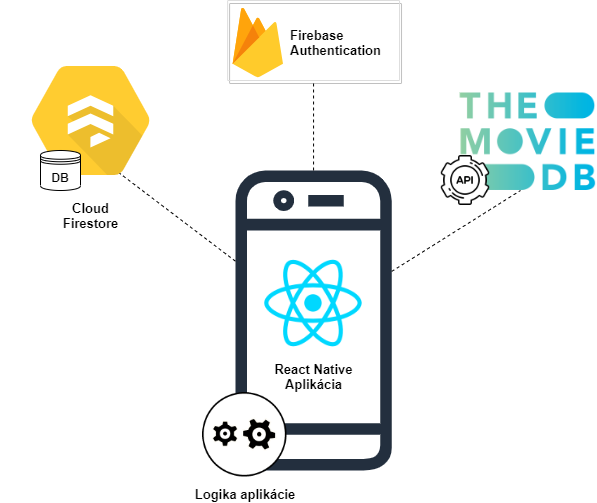
\includegraphics[height=10cm]{img/app-diagram.png}}%
           {\scriptsize}
	\caption{Znázornenie konceptu aplikácie}  
  \label{app-diagram}
\end{figure}

V ďalšej časti práce je návrh detailnejšie vizualizovaný pomocou vybraných UML diagramov. 

\pagebreak

\subsubsection{Diagramy prípadov použitia}
\begin{figure}[hbt!]
  \centering  
  \def\stackalignment{c}
	\stackunder{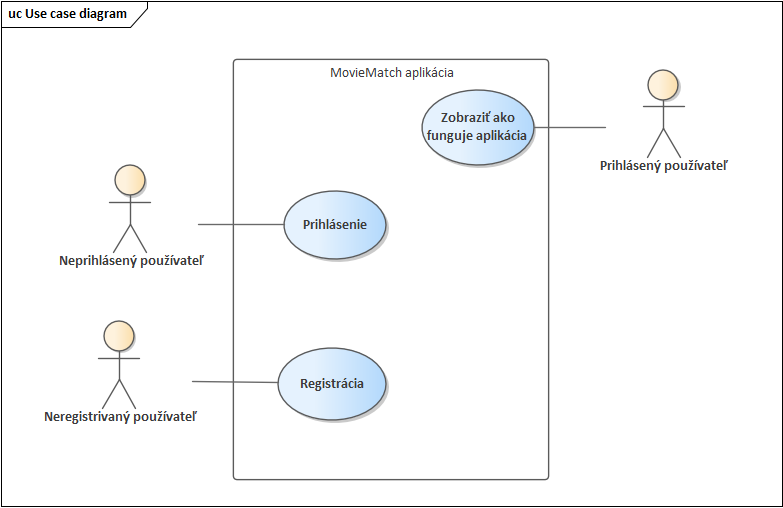
\includegraphics[height=10cm]{img/usecase1.png}}%
           {\scriptsize}
	\caption{Diagram prípadov použitia 1}  
  \label{usecase1}
\end{figure}

Na \hyperref[usecase1]{obrázku 8} môžeme vidieť, že aplikácia rozlišuje 3 základné role a to neregistrovaný používateľ a registrovaný (treba opravit diagram) resp. prihlásený používateľ. Neregistrovaný používateľ sa vie zaregistrovať pomocou zvolenej prezývky, emailu a hesla. Následne ho aplikácia rovno prihlási pričom mu zobrazí krátky návod na oboznámenie sa s aplikáciou. Na jeho konci je z populárnych titulov vygenerovaný úvodný dotazník, v ktorom je požívateľ vyzvaný, aby pomocou swipeovania vybral aspoň 15 filmových titulov ktoré sa mu páčia. To zabezpečí, že sa profil preferencií nainicializuje. Registrovaný používateľ sa vie prihlásiť pomocou emailu a hesla.
\pagebreak

\begin{figure}[hbt!]
  \centering  
  \def\stackalignment{c}
	\stackunder{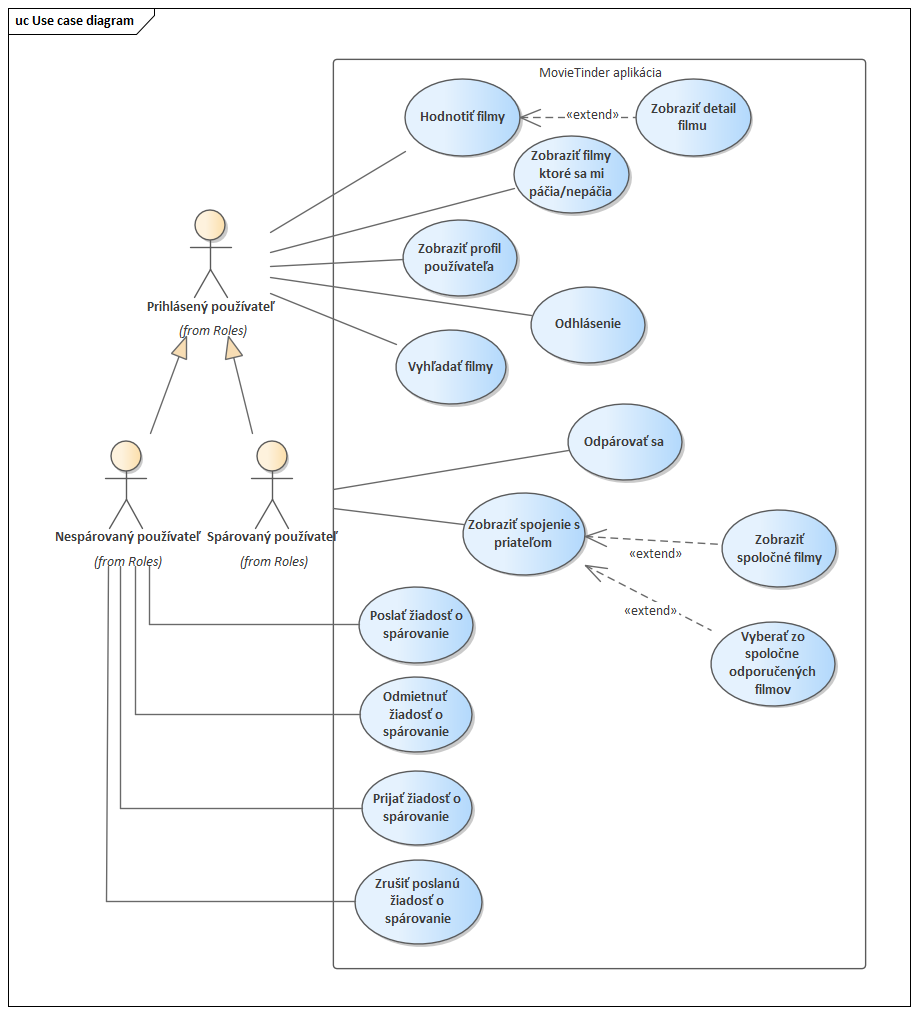
\includegraphics[width=15cm]{img/usecase2.png}}%
           {\scriptsize}
	\caption{Diagram prípadov použitia 2}  
  \label{usecase2}
\end{figure}
Na \hyperref[usecase2]{obrázku 9} máme detailnejší popis aplikácie po prihlásení používateľa. Prihlásený používateľ má možnosť hodnotiť filmy, prípadne si pozrieť detail aktuálne zobrazeného filmu. Tak isto si vie zobraziť filmy, ktoré sa mu páčili. Vie si tiež zobraziť svoj profil so základnými informáciami o jeho účte a odhlásiť sa z aplikácie. Po prihlásení môže používateľ nadobudnúť dve ďalšie podrole.

Nespárovaný používateľ vie poslať žiadosť o spárovanie inému používateľovi, ktorú v prípade neobdržania odpovede vie kedykoľvek zrušiť. Vďaka tomu sa vyhne situácií, kedy by sa zasekol v stave čakania na odpoveď. Po obdržaní takejto žiadosti, vie túto žiadosť odmietnuť alebo prijať. Prijatím sa automaticky spáruje s druhým používateľom a na základe ich profilov preferencií sa im vygenerujú spoločné odporúčané filmové tituly, ktoré vedia obaja používatelia hodnotiť. 

Každý spárovaný používateľ má možnosť si pozrieť aktuálne spojenie, hodnotiť v ňom filmy, pozerať si spoločné zhody a v neposlednom rade má možnosť sa odpárovať a následne spárovať s ďalším používateľom. 

\subsubsection{Diagram tried}
\begin{figure}[hbt!]
  \centering  
  \def\stackalignment{c}
	\stackunder{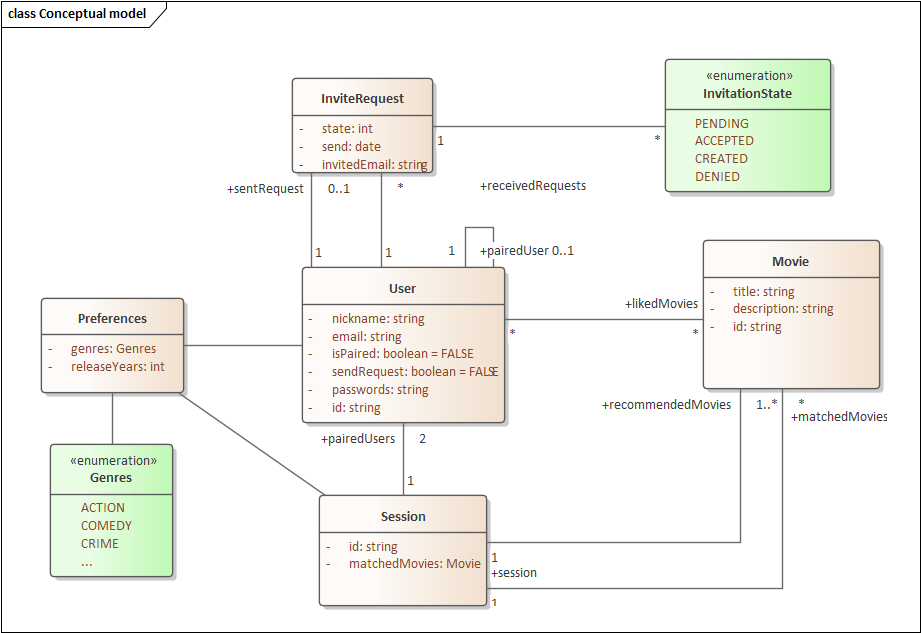
\includegraphics[width=15cm]{img/conceptualmodel.png}}%
           {\scriptsize}
	\caption{UML diagram tried}  
  \label{classdiagram}
\end{figure}
\hyperref[classdiagram]{Obrázok 10} zobrazuje diagram tried aplikácie. Ústredným prvkom našej aplikácie je trieda User, ktorá reprezentuje používateľov tohto systému. Používateľ vie byť v spojení s najviac jedným ďalším používateľom pomocou triedy Session. Táto trieda predstavuje spojenie medzi dvoma používateľmi a na základe preferencií, ktoré majú používatelia, sa v tomto spojení generujú odporúčané filomové tituly. Okrem toho je možné si v danom spojení pozrieť filmy, ktoré obaja používatelia hodnotili pozitívne. Samotný používateľ má vlastné spojenie s triedou Movie, vďaka ktorému si vie zobraziť filmy, ktoré sa mu páčili.

Každý používateľ vie obdržať viacero pozvánok na spojenie, ktoré sú reprezentované triedou InviteRequest, avšak prijať vie práve jednu. Odoslať vie tak isto iba jednu, čo zabraňuje situácii, kedy by viacero používateľov prijalo pozvánku jedného používateľa. Po odoslaní je pozvánka v stave PENDING kým na ňu príjemca neodpovie. Po prijatí pozvánky sa medzi používateľmi vytvorí spojenie, v ktorom si spolu vyberajú filmové tituly až kým sa nerozhodnú toto spojenie ukončiť. Trieda Preferences je dôležitým prvkom v sýstéme odporúčaní, keďže pomocou nej sa generujú odporúčané tituly pre jednotlivé spojenia.

%Význam väčšiny atribútov je z ich názvu jasný, preto spomenieme len tie, ktoré považujeme za potrebné objasniť. Pri triede User atribút isPaired vyjadruje, či daný používateľ je spárovaný s iným používateľom a atribút sendRequest, či daný používateľ poslal žiadosť o spárovanie inému používateľovi. 

\section{Implementačná časť}
V tejto časti práce sa pozrieme na celý implementačný proces od úvodného nastavenia a inštalácie potrebných nástrojov, až po konkrétne časti implementácie aplikácie.

\subsection{Uvodná inštalácia a nastavenia}
Predtým ako sme začali s programovaním aplikácie, bolo treba nastaviť a nainštalovať potrebné nástroje.
\subsubsection{VSCode}
Ako vývojové prostredie sme si vybrali Visual Studio Code. Výber vychádzal hlavne z osobných preferencií a dostupnosti množstva užitočných rozšírení. Stiahli sme ho z \href{https://code.visualstudio.com/download}{oficiálnej stránky} vývojára.
\subsubsection{React Native}
\begin{itemize}
{\item Ako prvé bolo treba nainštalovať Node.js z jeho \href{https://nodejs.org/en/download/}{oficiálnej stránky}. Kvôli stabilite sme stiahli LTS verziu. Inštalácia obsahuje aj predvolený package manager npm.} 
{\item Keďže sme počas implementácie uprednostnili yarn namiesto npm, bolo ho treba najprv doinštalovať pomocou npm príkazu \textit{npm install -g yarn}.} 
{\item Potom sme pomocou yarnu a príkazu \textit{yarn global add expo-cli}, nainštalovali Expo CLI.} 
{\item Posledným krokom k úspešnému spusteniu aplikácie je nainštalovanie emulátora, ktorý bude slúžiť ako virtuálne prostredie pre spustenie našej aplikácie počas programovania. Expo CLI síce podporuje aj spustenie na reálnom zariadení, emulátor je však pohodlnejšie riešenie. V našom prípade, keďže sme aplikáciu programovali primárne pre Android OS, nám nato poslúži \href{https://developer.android.com/studio}{Android Studio}, ktoré túto funkcionalitu obsahuje.}
\end{itemize}

V tomto bode by sme mali byť schopný inicializovať aplikáciu príkazom \textit{expo init nazovProjektu}.
Treba dodať, že občas sa počas inštalácie Expo CLI cez npm môže vyskytnúť chyba, kedy sa nepridá expo do systému ako environment variable. Následne po zadaní príkazu, príkazový riadok hlási chybu, že nepozná daný príkaz. To sa stalo aj v našom prípade. Riešením je buď ju pridať manuálne (čo nemusí vždy pomôcť), alebo preinštalovať Node.js a nainštalovať Expo CLI pomocou npm znova. Po preinštalovaní už príkaz funguje, vďaka čomu sme nainicializovali a vytvorili našu aplikáciu. 

\subsubsection{Firebase}
Keďže firebase je platforma vyvinutá Googlom, prihlasuje sa do nej pomocou google účtu. Po prejdení do konzoly, čo je časť kde sa dá vytvoriť a následne pracovať s projektom, si vytvoríme projekt s názvom našej aplikácie MovieTinderApp. Vo vnútri projektu zvolíme OS aplikácie, na ktorú ho chceme napojiť, v našom prípade Android OS.  
\begin{figure}[hbt!]
  \centering  
  \def\stackalignment{c}
	\stackunder{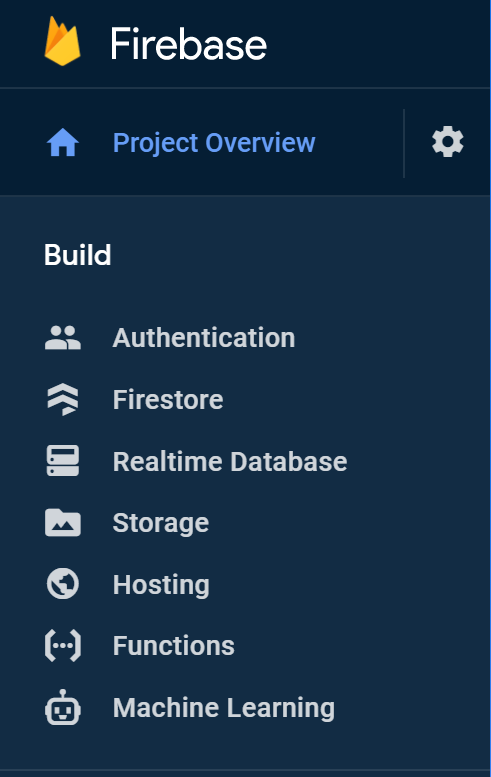
\includegraphics[height=7cm]{img/firebaseconsole.png}}%
           {\scriptsize}
	\caption{Firebase console menu}  
  \label{fireconsole}
\end{figure}
Po zadaní povinných údajov ako názov aplikácie a názov android package, sa nám  vygeneruje objekt s konfigruračnými údajmi. Ten si skopírujeme a vložíme do novovytvoreného súboru v našej aplikácií s názvom keys.js. Tam budeme uchovávať všetky potrebné citlivé údaje ako napríklad API kľúče a podobne. Na \hyperref[classdiagram]{obrázku 11} vidíme ukážku menu z firebase console. Okrem týchto funkcií poskytuje aj všeobecný prehľad o aplikácií a rôzne štatistiky a analytické funkcie. 

Posledným krokom inštalácie je pridanie firebase cez yarn príkazom \textit{yarn add firebase} a následné pridanie inicializácie v hlavnom súbore App.js pridaním \textit{firebase.initializeApp(config);}
\subsubsection{Firebase authentication}
Firebase ponuká mnoho rôznych spôsobov autentifikácie používateľa. My sme zvolili klasický pomocou emailu a hesla. Vo firebase console sme v záložke authentication povolili metódu prihlasovania email/password. 
\subsubsection{TMDb}
Na využívanie databázy filmových titulov TMDb resp. jej API, bolo potrebné si na webstránke služby založiť účet. Následne nám bol vygenerovaný API kľúč, ktorý sme vložili do spomínaného súboru keys.js. 
\subsubsection{GitHub}
Na zálohovanie zdrojového kódu sme použili \href{https://github.com/}{GitHub}, čo je voľne dostupná webová služba, ktorá poskytuje zálohu kódu, jeho verzionovanie prípadne sledovanie zmien a mnohé iné užitočné funkcie. Je jednou z najpopulárnejších služieb s týmto zameraním. Repozitár s našou aplikáciou je zverejnený na odkaze na \hyperref[ghqrcode]{obrázku nižšie}. 

\begin{figure}[hbt!]
  \centering   
  \def\stackalignment{c}
	\stackunder{
\includegraphics[height=5cm]{img/github_qr.png}}%
           {\scriptsize%
            \url{https://github.com/adamt1312/MovieMatchApp}}
	\caption{QR kód GitHub repozitára aplikácie}  
  \label{ghqrcode}
\end{figure}
\subsection{Štruktúra obrazoviek inštalácia a nastavenia}
\subsubsection{React Navigation}
\subsection{Prihlasovanie a registrácia}
\subsection{Mechanizmus párovania}
\subsection{Odporúčací algoritmus}










